%!TEX root=main.tex

\section{Results} \label{sec:results}
In this section, we explain our results with HMM and NN model.

\begin{figure}[t]
  \centering
  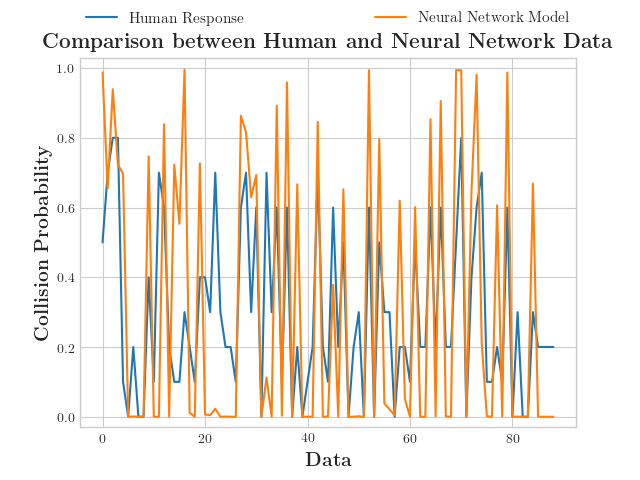
\includegraphics[width=\linewidth]{figures/nn_result.png}
  \caption{Comparisons between human responses and neural network model prediction. The Pearson correlation between the two data is $0.69$, which indicates a good linear relationship between neural network model and human decision making.}
  \label{fig:nn_raw_result}
\end{figure}

\begin{figure}[t]
	\begin{subfigure}[t]{1\linewidth}
		\centering
		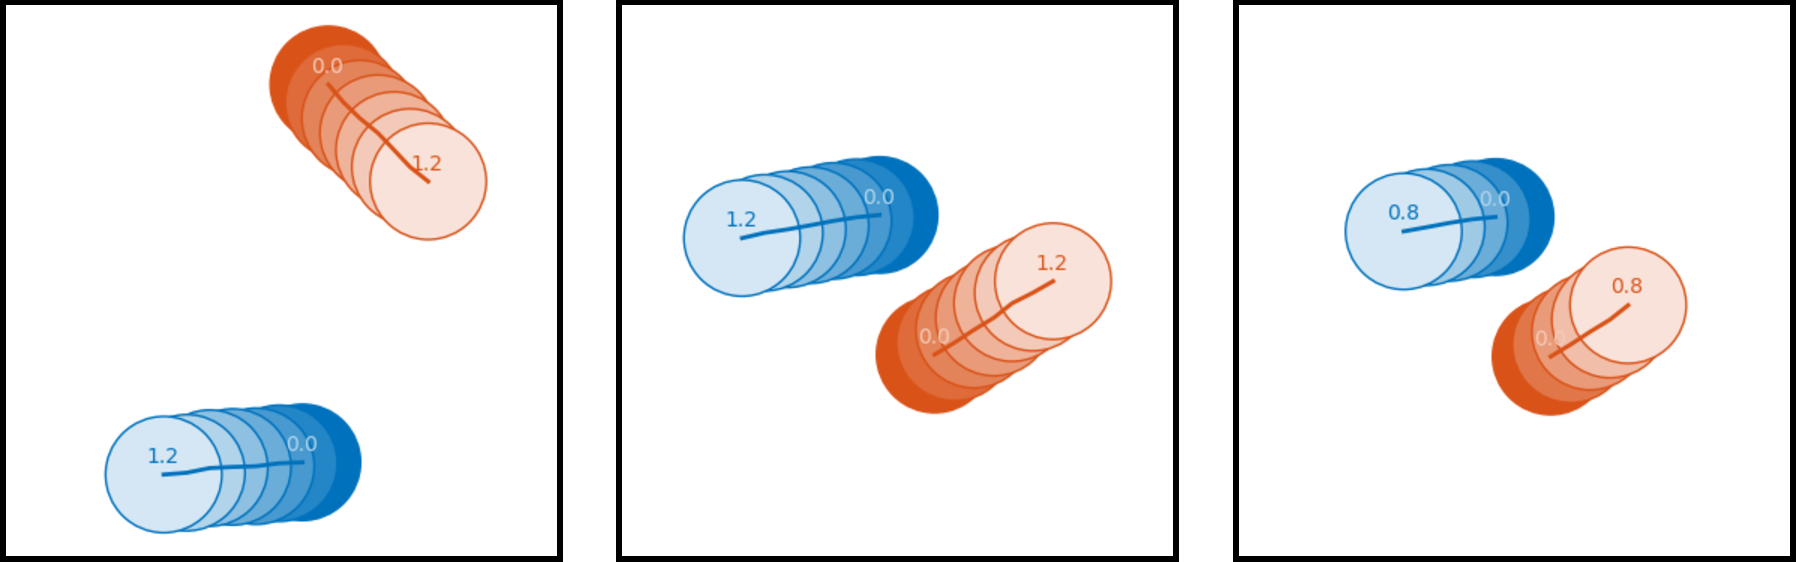
\includegraphics[width=0.95\linewidth]{figures/agree.pdf}
		\caption{Agreed Test Data Points}
		\label{fig:nn-agree}
	\end{subfigure}
    \\
    \par\bigskip
	\begin{subfigure}[t]{1\linewidth}
		\centering
		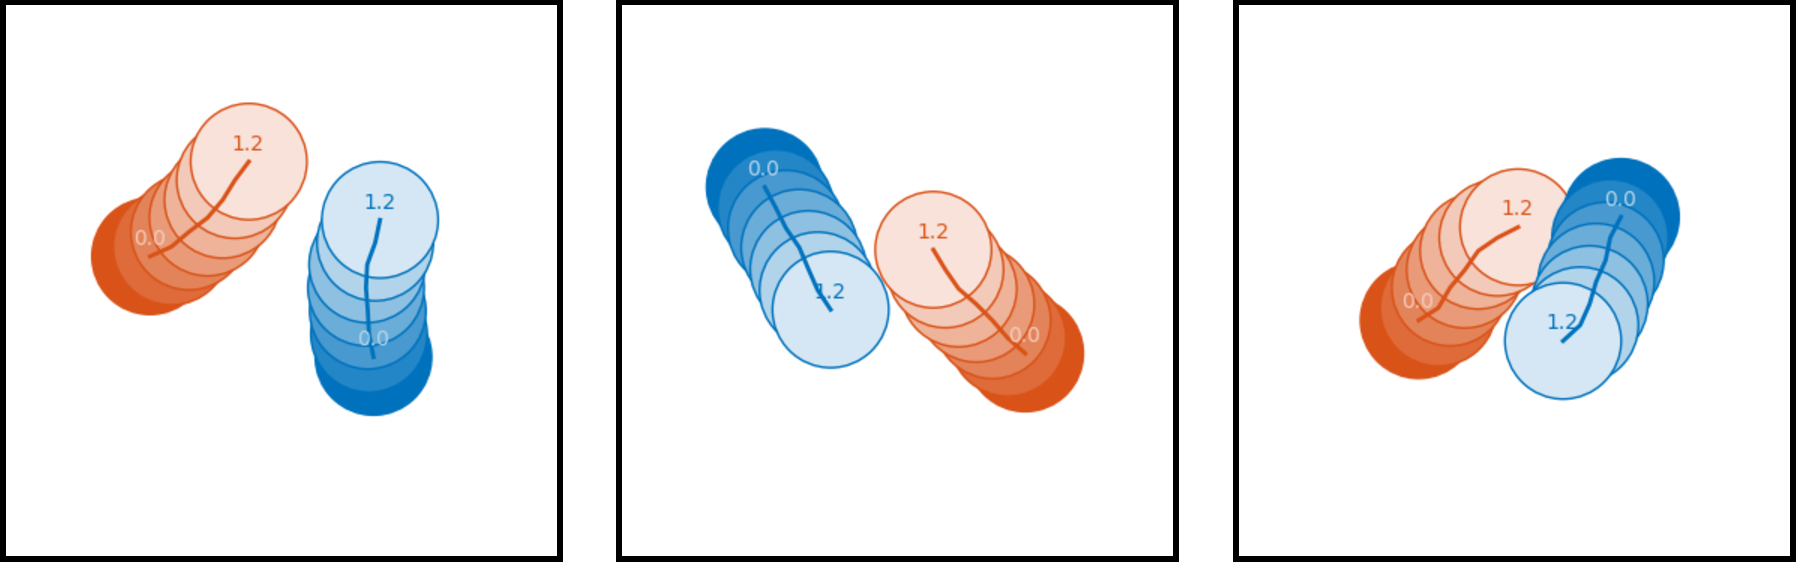
\includegraphics[width=0.95\linewidth]{figures/disagree.pdf}
		\caption{Disagreed Test Data Points}
		\label{fig:nn-disagree}
	\end{subfigure}
	\caption{(a) Test data points that both human and neural network model predict to be zero collision. (b) Test data points that human and the model strongly disagree. Left: $P_{collision} = 0.3$ (human response) vs $1.0$ (neural network prediction probability). Center: $0.7$ vs $0.1$. Right: $0.7$ vs $0.0$.}
	\label{fig:nn-analysis}
\end{figure}

\begin{figure}[t]
  \centering
  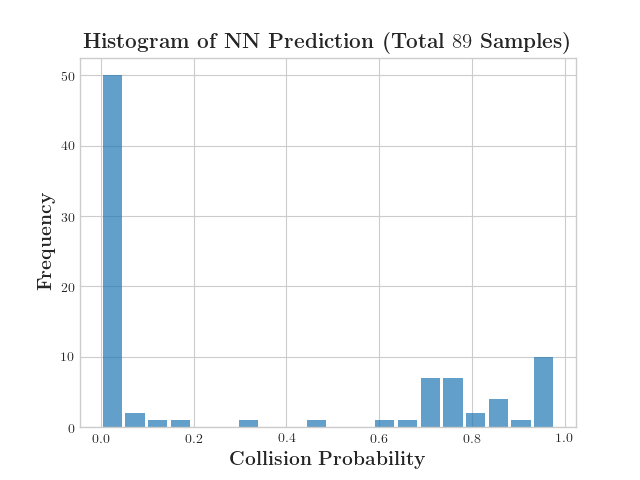
\includegraphics[width=\linewidth]{figures/nn_hist.png}
  \caption{Histogram of neural network prediction on the test dataset. Similar to the human responses, the result shows a bias toward no-collision. The neural network model is more confident than the human in its' collision predictions.}
  \label{fig:nn_hist}
\end{figure}

\subsection{Neural Network}
We consider two neural network models: one without bootstrapping and the other with bootstrapping. 
Compared to the model without bootstrapping, the model with bootstrapping provides additional information about uncertainty.
In this section, we first demonstrate our result with neural network without bootstrapping and then discuss further analysis with uncertainty.

\begin{figure}[t]
  \centering
  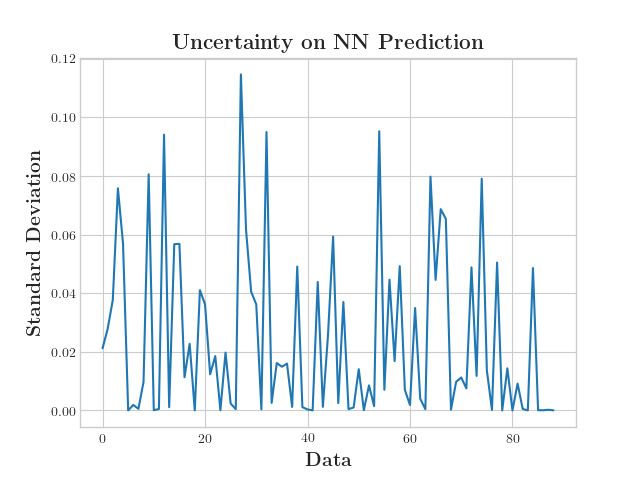
\includegraphics[width=\linewidth]{figures/uncertainty.png}
  \caption{Uncertainty of the neural network predictions on the test dataset. Peaks mostly correspond to ambiguous situations as depicted in~\cref{fig:nn-uncertain-data}, which displays datapoint $27$.}
  \label{fig:nn-uncertainty}
\end{figure}

\begin{figure}[t]
  \centering
  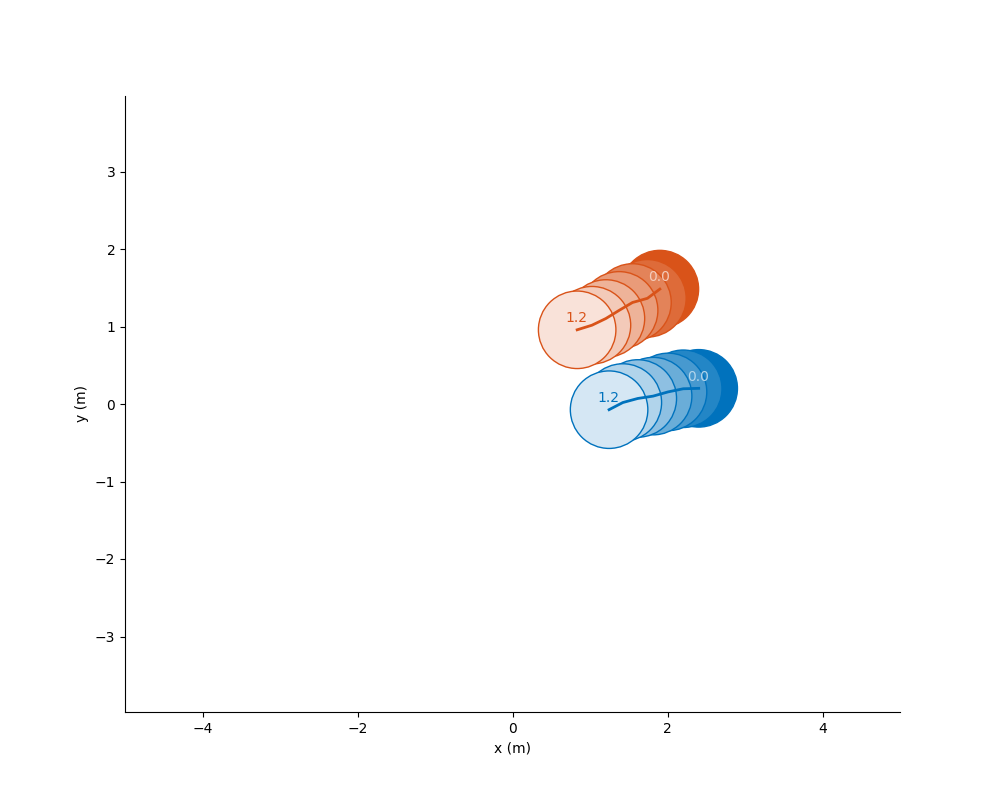
\includegraphics[width=\linewidth]{figures/unceratin_data.png}
  \caption{Test data point with id $27$ that both neural network and human are confused about. The neural network indicates confusion by the standard deviation (i.e., uncertainty) of $0.11$. The test participants have rated  $0.6$ collision probability, which is close to a random guess ($0.5$).}
  \label{fig:nn-uncertain-data}
\end{figure}

\begin{figure}[t]
  \centering
  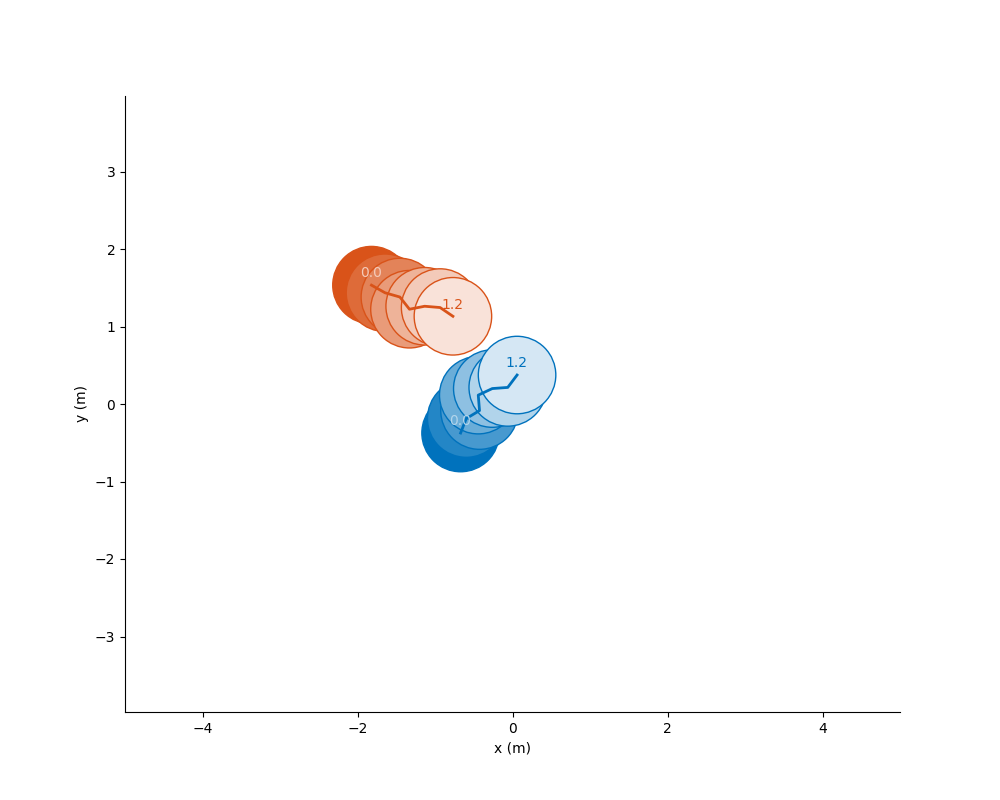
\includegraphics[width=\linewidth]{figures/noise_data.png}
  \caption{The test data with Gaussian noise. Gaussian noise has never been observed in the neural network's training dataset. On the novel observation with Gaussian noise (wiggly trajectory), the neural networks' predictions are more likely to be erroneous. The uncertainty-aware model can identify these novel scenarios and similar to the human \textit{know what it does not know}.}
  \label{fig:noise-data}
\end{figure}

% \begin{figure}[t]
% 	\begin{subfigure}[t]{1\linewidth}
% 		\centering
% 		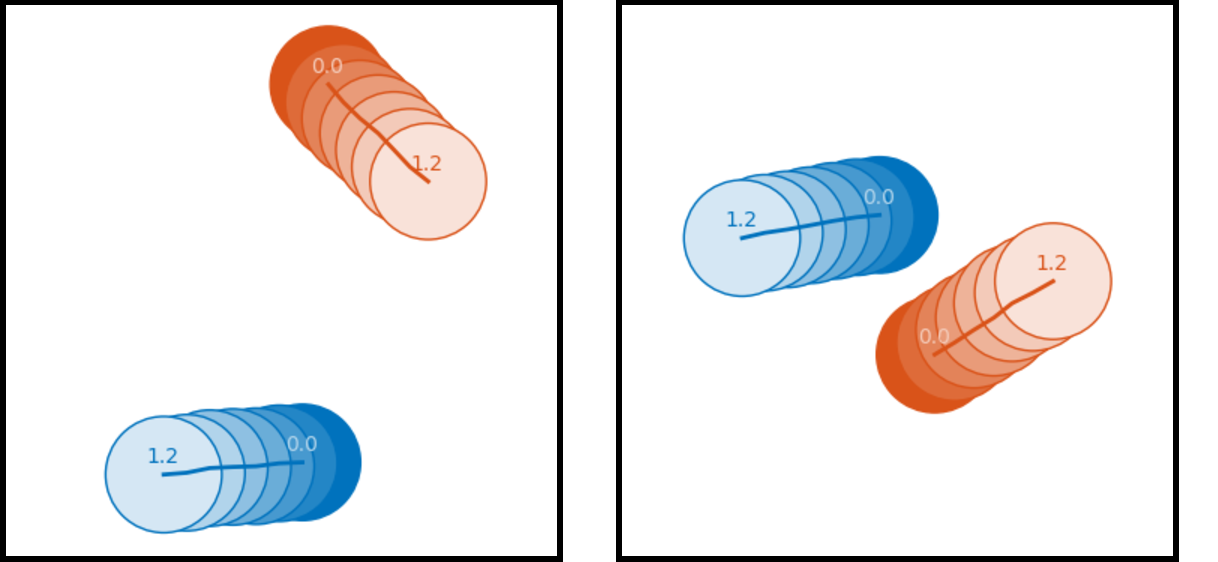
\includegraphics[width=0.95\linewidth]{figures/hmm_agree.pdf}
% 		\caption{Agreed Test Data Points for HMM}
% 		\label{fig:hmm-agree}
% 	\end{subfigure}
%     \\
%     \par\bigskip
% 	\begin{subfigure}[t]{1\linewidth}
% 		\centering
% 		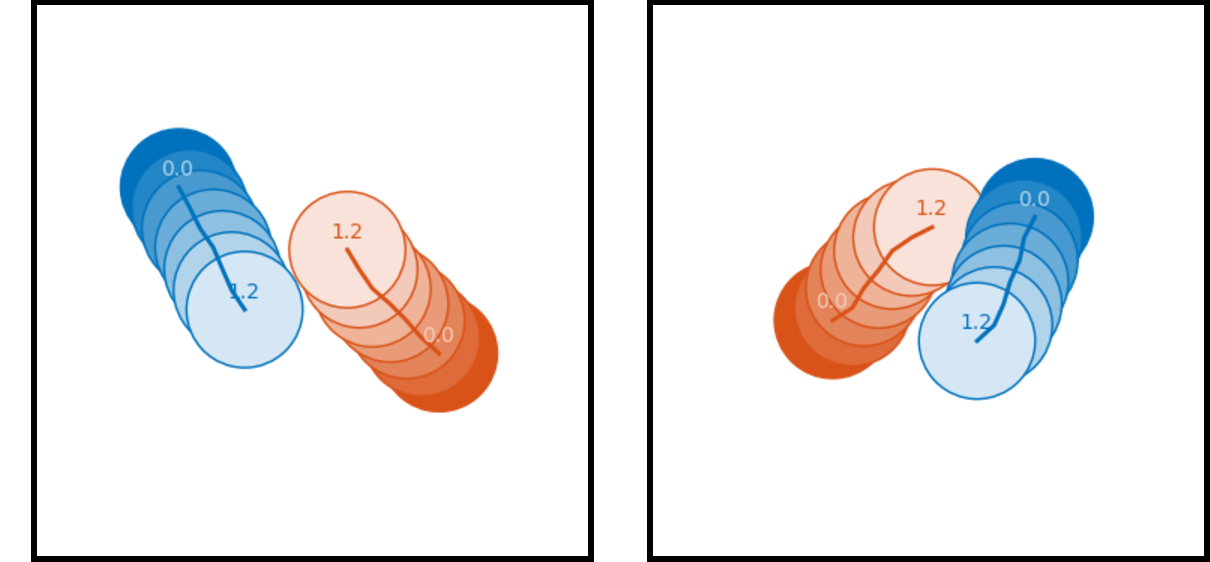
\includegraphics[width=0.95\linewidth]{figures/hmm_disagree.pdf}
% 		\caption{Disagreed Test Data Points for HMM}
% 		\label{fig:hmm-disagree}
% 	\end{subfigure}
% 	\caption{(a) Test data points that both human and HMM predict to be no collision. (b) Test data points that human and HMM strongly disagree. Left: $P_{collision}=0.7$ (human response) vs no-collision (HMM prediction). Right: $0.7$ vs no-collision.}
% 	\label{fig:hmm-agree-disagree}
% \end{figure}

\subsubsection{Neural Network without Bootstrapping}
We first trained the network with the aforementioned training procedure.
Then we \textit{tested} the trained model using the data used to collect human responses\footnote{We hereafter refer the data used to collect human responses as \textit{test} dataset.}.

The comparison between the (normalized) human ratings and predicted collision probabilities by the neural network model is shown in \cref{fig:nn_raw_result}.
The Pearson correlation between the two data is $0.69$\footnote{A correlation of 0 means no linear relationship. A correlation of 1 or -1 means a strong positive linear or negative relationship.}, which shows a good linear relationship between the two. Motivated by their linear relationship, we generate the histogram of the neural network model's prediction to see whether it also shows a bias toward the no-collision similar to human responses (see \cref{fig:human-data-collection}).
\Cref{fig:nn_hist} shows the histogram of the neural network prediction on the test dataset. Similar to the human responses, it does show a bias toward the no-collision. 
However, compared to the human responses, it has a much stronger bias toward the no collision probability. 

We delve deeper into the neural network model analysis by looking at test data points that human and the model strongly agree or disagree.
\cref{fig:nn-agree} shows test data points that both human and neural network model predicts the same collision probability of zero. 
These data points commonly show a trend that the two agents are heading to very different directions each other with sufficiently far distances. 
It is plausible for both humans and neural network model that the trend is a good reason to decide why the agents are not likely to collide.
On the other hand, \cref{fig:nn-disagree} describes another test data points that human and the model predict opposite decision (e.g., human predicts to be likely no collision but neural network model predicts to be collision).
Based on these test data points, humans are likely to predict collision if the two agents are close. However, if the two agents tend to move in a same direction, then human tends to give no collision.
However, the neural network model seems to be more sensitive to the orientation instead of the distance.% So if bad why is it? what can be done better?
\\

\subsubsection{Neural Network with Bootstrapping}
Uncertainty about NN model's prediction provides useful information such that we could use to understand what data points that the model is confused at. 
The uncertainty in its prediction is measured by the bootstrapping~\cite{Osband2016, Lakshmi2016}. 
The uncertainty about collision probability on test data points is shown in \cref{fig:nn-uncertainty}. Also, \cref{fig:nn-uncertain-data} shows the test data point that the NN model is the most confused at.
The model predicted a collision probability of $0.76$ with a standard deviation of $0.11$. 
It is understandable as a small orientation change could cause either collision or no collision.
This is also an interesting result because a human would be also confused at the same data point. Thus, we have adapted the neural network model to have a closer decision making to humans, compared to the neural network model without uncertainty.

\subsubsection{Neural Network Model with a Novel Data Point}
When a human is experienced with a new problem, he or she would have a little confident in solving the problem.  
Would the same capability exist in the neural network model? 
Would the uncertainty estimate provide the neural network model to be similar to a human?
To answer our questions, we generated a new data that significantly differs from our train dataset. 
Compared to the train dataset, which is noise-free, the new data has a large noise in its heading: for each time, we added a Gaussian noise with a mean of $0$ degree and a standard deviation of $30$ degree to each agent's heading.
The data is shown in \cref{fig:noise-data}. Interestingly, the neural network model with uncertainity predicted a collision probability of $0.69$ and a standard deviation (i.e., uncertainty) of $0.28$. 
Considering that the most biggest standard deviation in the test dataset was $0.11$ (see \cref{fig:nn-uncertainty}), the uncertainty on the new data is large. 
This result is desirable as we would expect the network to output a large uncertainty because the data significantly differs to the ones in the train dataset.
Considering a human would be also uncertain about a new situation that he or she never has experienced before, this result conveys that the neural network with uncertainty resembles better a human decision making compared to the model without uncertainty.

\subsection{Hidden Markov Model}
% \subsubsection{Limitations of the H
The HMM is able to model the closeness between agents to a limited degree.

Although it captures the notion of "small" and "large" distances given the orientations and positions of the agents, it is unable to model increasing and decreasing distances without any additional observations. It lacks the richness of human experiences to "forward" its physics engine. The model also doesn't understand agent intention: it lacks an intuitive psychology model and assumes that agent will continue going in the same direction. \\
Furthermore, the solution is implemented using the most likely orientation state. The implementation does not consider the global structure of observations, the neighboring states (with respect to timing), and the length of the observations. This type of "instantaneous optimality" can be problematic as it does not capture the overall sequential structure of the problem. \\
Nevertheless, the HMM allows for easy adaptation to the collected human data. By simply varying the prior $Pr(d) = i \forall d \in [0,9]$, where $d$ is the euclidean distance between the two agents are we able to have some intuition behind how human reason about collision physics and intention.~\Cref{fig:hmm-coll-pred} shows that the uniform prior on state probabilities matches the actual count of collisions across the $89$ experiments. Changing the prior to favor fewer collisions allows the frequency counts of the HMM to be more similar to the human results. \\
From this comparison, we can make a general conclusion that humans are more likely to predict collisions, when the observed distance in between the pedestrians in low. Intuitively, this makes sense. Additionally, the HMM was able to imitate the bias humans have towards predicting no collision and a small second bias in a collision score between $5-7$.

\begin{figure}[t]
	\begin{subfigure}[t]{1\linewidth}
		\centering
		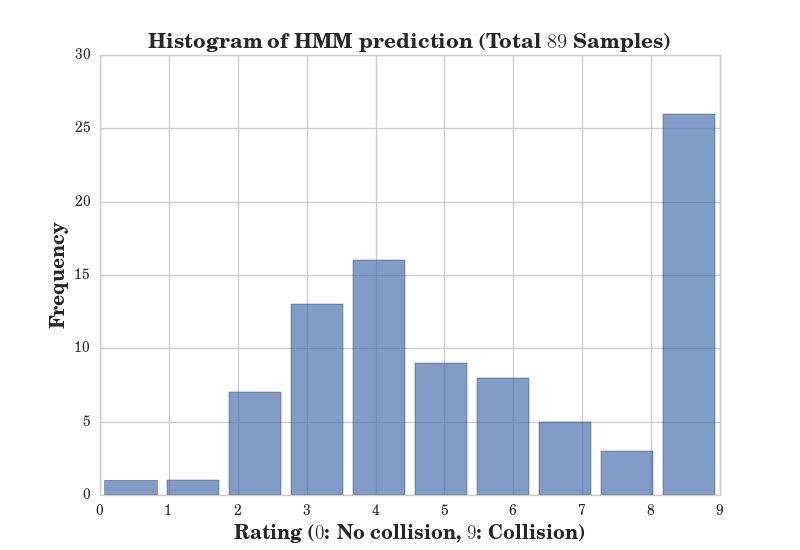
\includegraphics[width=0.95\linewidth]{figures/hmm_prior.png}
		\caption{Before posterior update.}
		\label{fig:hmm-coll-pred-prior}
	\end{subfigure}
	\begin{subfigure}[t]{1\linewidth}
		\centering
		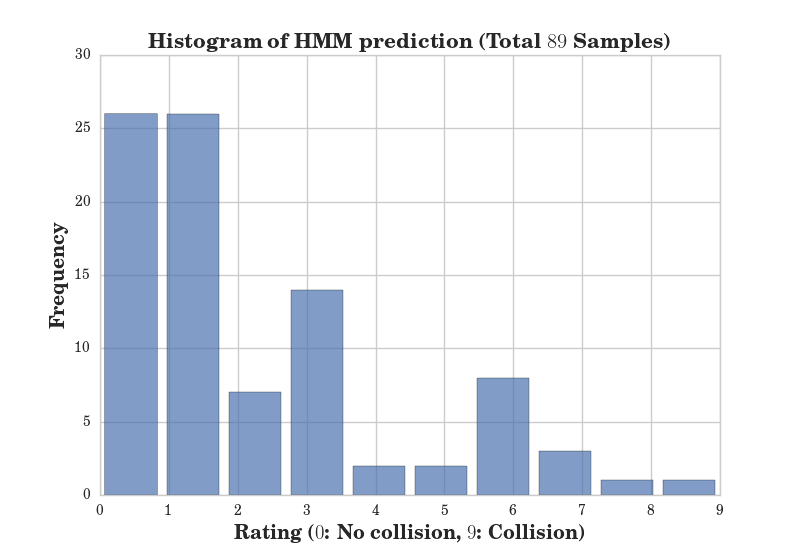
\includegraphics[width=0.95\linewidth]{figures/hmm_posterior.png}
		\caption{After posterior update.}
		\label{fig:hmm-coll-pred-post}
	\end{subfigure}
	\caption{HMM collision prediction. The HMM predicts a collision rating on the scale from $0$ to $9$ for $89$ sample trajectories. The HMM inference with default parameters in~\cref{fig:hmm-coll-pred-prior} deviates strongly from the human prediction in~\cref{fig:histogram-human-data}. We then adapt the parameters in~\cref{fig:hmm-coll-pred-post} to imitate human decision making. Similar to the human prediction, the HMM after posterior update has a bias towards "no collision" and has a low second peak around collision likelihood $5-7$.}
	\label{fig:hmm-coll-pred}
\end{figure}
\\

% This leads to an interesting discussion of where the collisions are being identified in each experiment. \dkXX{Insert graphics similar to fig 9 here.}.

% \iffalse
% \begin{figure}[t]
% 	\begin{subfigure}[t]{1\linewidth}
% 		\centering
% 		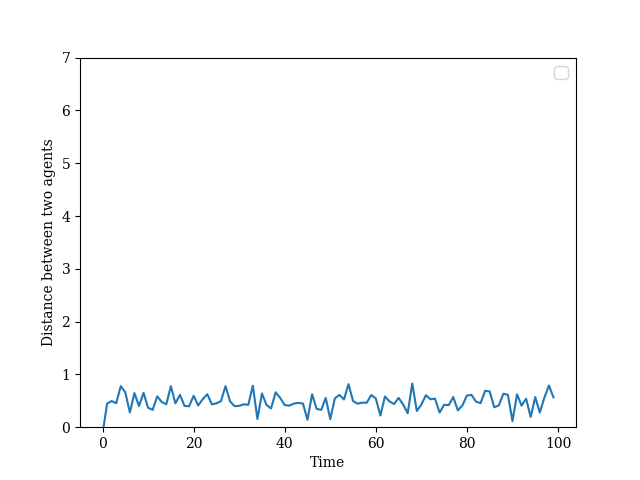
\includegraphics[scale=0.50]{figures/hmm_e_0.png}
% 		\caption{Sampling the distance HMM in experiment 0.}
% 		\label{fig:nn}
% 	\end{subfigure}
%     \\
%     \par\bigskip
% 	\begin{subfigure}[t]{1\linewidth}
% 		\centering
% 		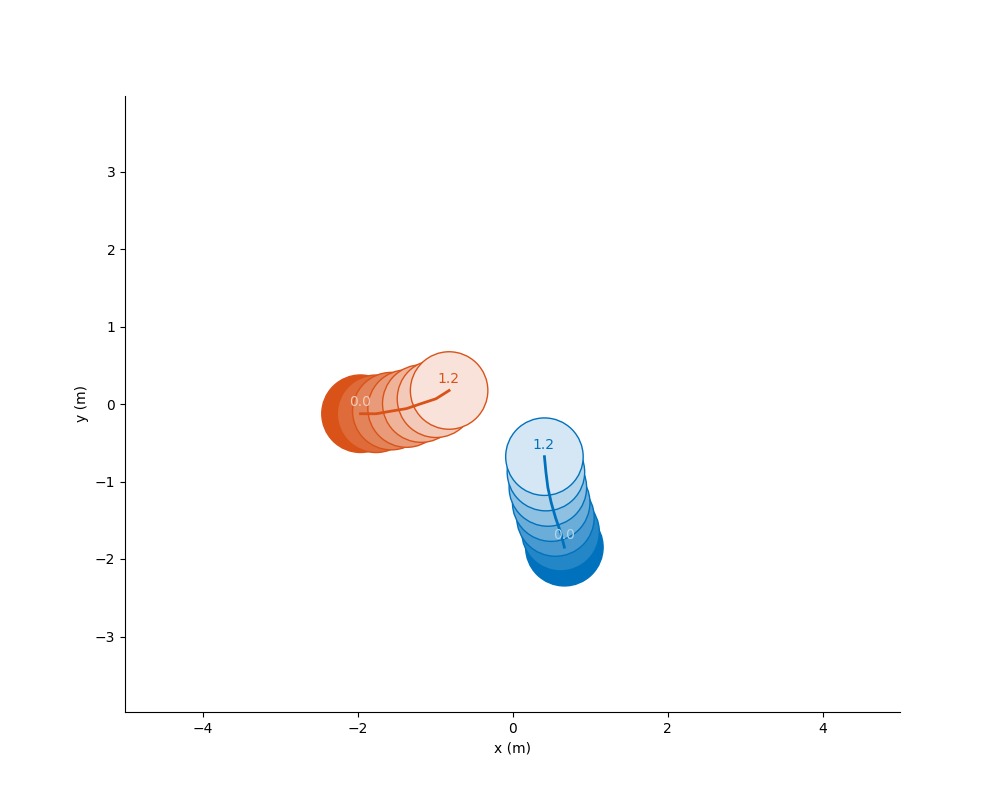
\includegraphics[scale=0.25]{figures/course_966_e_00_t_05.png}
% 		\caption{The five timesteps of information given to the HMM.}
% 		\label{fig:nn-bootstrap}
% 	\end{subfigure}
% 	\caption{Experiment 0: HMM results against the observations. In this scenario, it looks like the two agents are very close to colliding: given their heading information, it seems like their paths will intersect.}
% 	\label{fig:nn-overview}
% \end{figure}

% \begin{figure}[t]
% 	\begin{subfigure}[t]{1\linewidth}
% 		\centering
% 		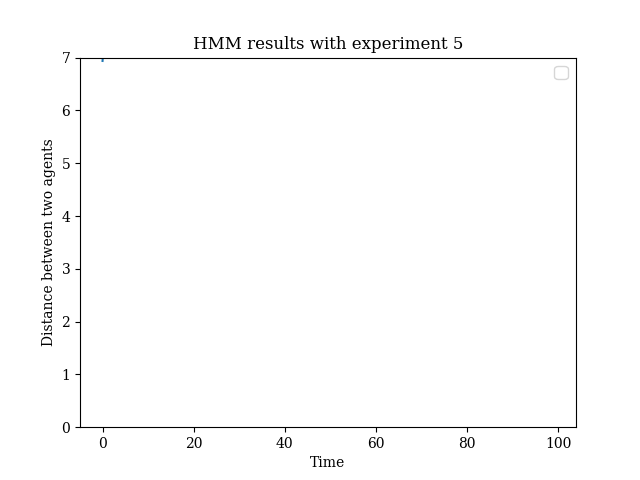
\includegraphics[scale=0.50]{figures/hmm_e_5.png}
% 		\caption{Sampling the distance HMM in experiment 0.}
% 		\label{fig:nn}
% 	\end{subfigure}
%     \\
%     \par\bigskip
% 	\begin{subfigure}[t]{1\linewidth}
% 		\centering
% 		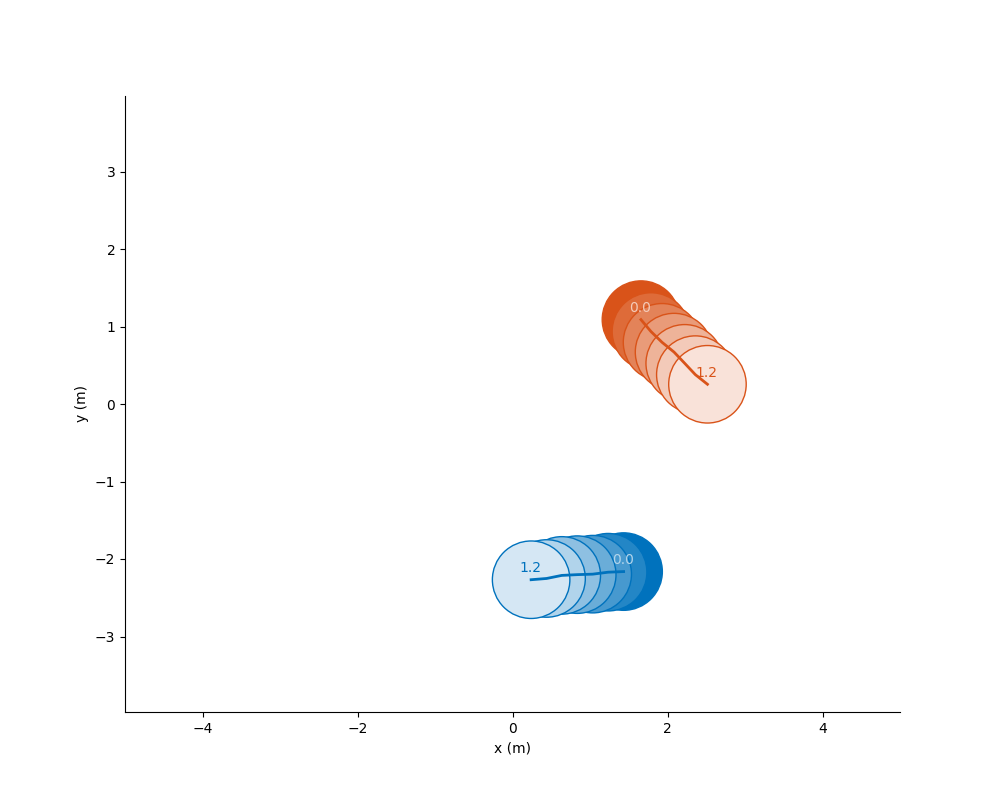
\includegraphics[scale=0.25]{figures/course_966_e_05_t_05.png}
% 		\caption{The five timesteps of information given to the HMM.}
% 		\label{fig:nn-bootstrap}
% 	\end{subfigure}
% 	\caption{HMM results against the observations. }
% 	\label{fig:nn-overview}
% \end{figure}

% \begin{figure}[t]
% 	\begin{subfigure}[t]{1\linewidth}
% 		\centering
% 		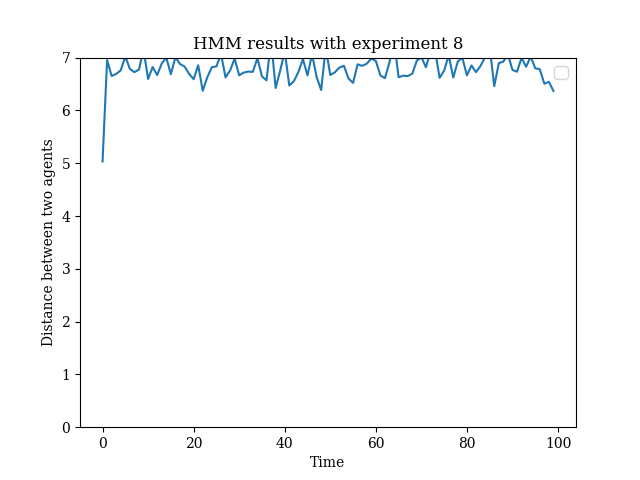
\includegraphics[scale=0.50]{figures/hmm_e_8.png}
% 		\caption{Sampling the distance HMM in experiment 0.}
% 		\label{fig:nn}
% 	\end{subfigure}
%     \\
%     \par\bigskip
% 	\begin{subfigure}[t]{1\linewidth}
% 		\centering
% 		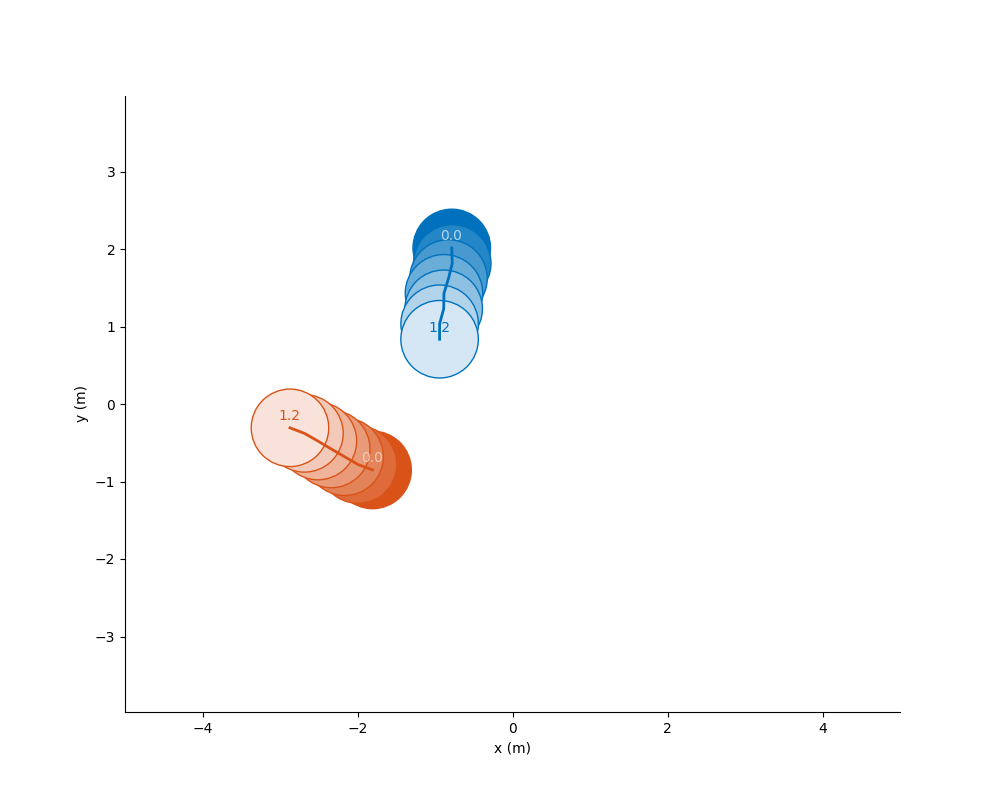
\includegraphics[scale=0.25]{figures/course_966_e_08_t_05.png}
% 		\caption{The five timesteps of information given to the HMM.}
% 		\label{fig:nn-bootstrap}
% 	\end{subfigure}
% 	\caption{HMM results against the observations.}
% 	\label{fig:nn-overview}
% \end{figure}

% \begin{figure}[t]
% 	\begin{subfigure}[t]{1\linewidth}
% 		\centering
% 		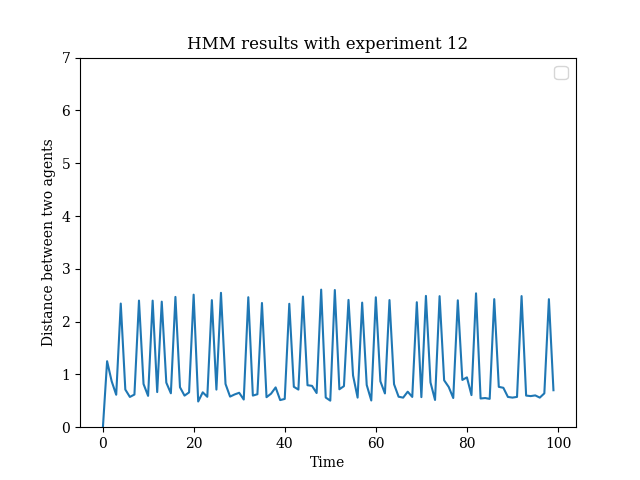
\includegraphics[scale=0.50]{figures/hmm_e_12.png}
% 		\caption{Sampling the distance HMM in experiment 0.}
% 		\label{fig:nn}
% 	\end{subfigure}
%     \\
%     \par\bigskip
% 	\begin{subfigure}[t]{1\linewidth}
% 		\centering
% 		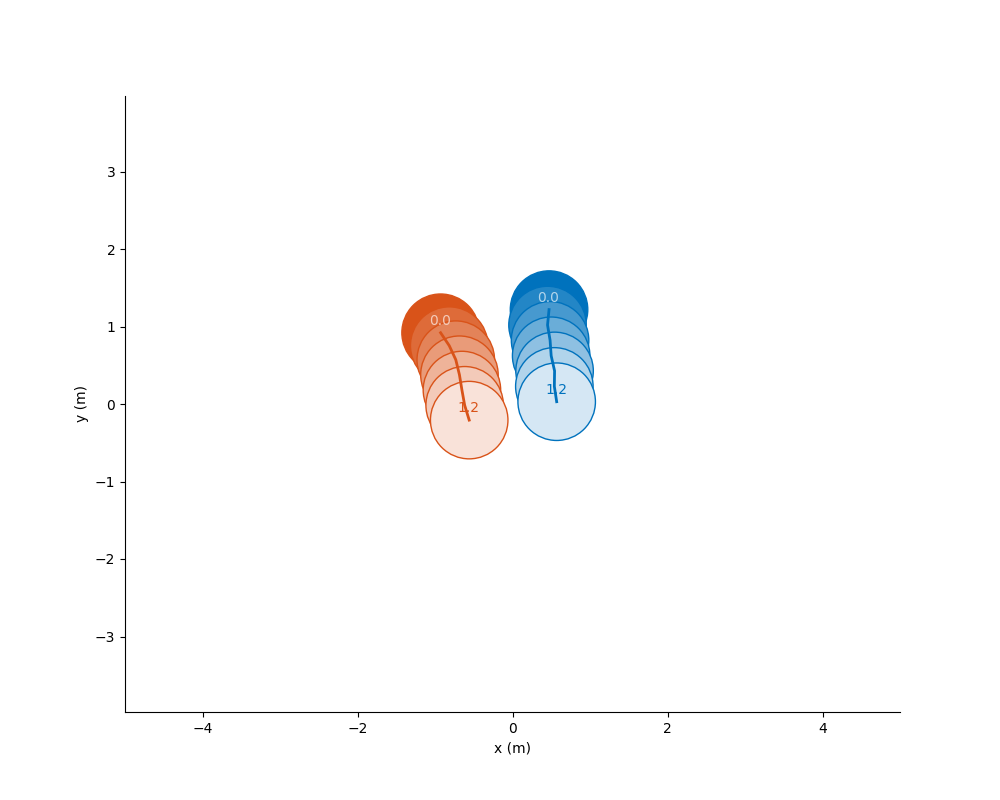
\includegraphics[scale=0.25]{figures/course_966_e_12_t_05.png}
% 		\caption{The five timesteps of information given to the HMM.}
% 		\label{fig:nn-bootstrap}
% 	\end{subfigure}
% 	\caption{HMM results against the observations.}
% 	\label{fig:nn-overview}
% \end{figure}

% \begin{figure}[t]
% 	\begin{subfigure}[t]{1\linewidth}
% 		\centering
% 		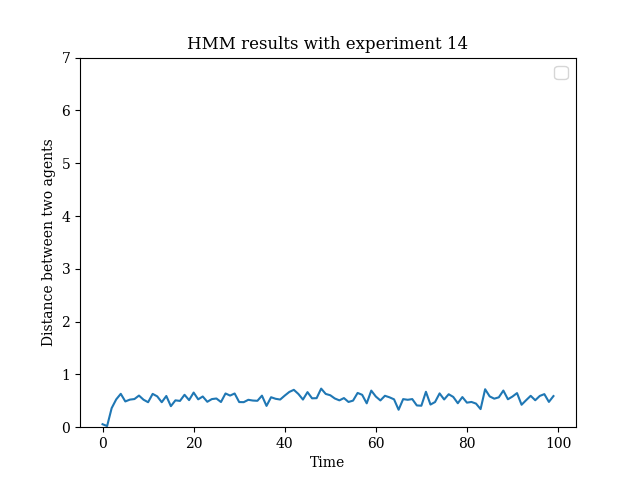
\includegraphics[scale=0.50]{figures/hmm_e_14.png}
% 		\caption{Sampling the distance HMM in experiment 0.}
% 		\label{fig:nn}
% 	\end{subfigure}
%     \\
%     \par\bigskip
% 	\begin{subfigure}[t]{1\linewidth}
% 		\centering
% 		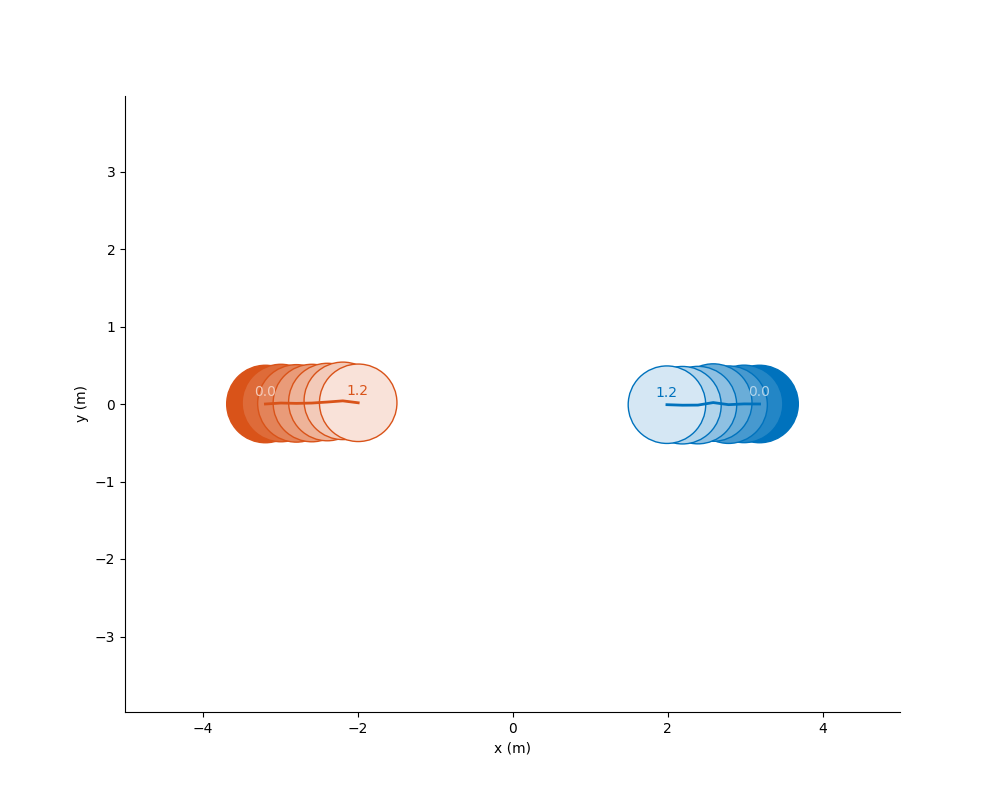
\includegraphics[scale=0.25]{figures/course_966_e_14_t_05.png}
% 		\caption{The five timesteps of information given to the HMM.}
% 		\label{fig:nn-bootstrap}
% 	\end{subfigure}
% 	\caption{HMM results against the observations.}
% 	\label{fig:nn-overview}
% \end{figure}
% \fi